\subsection{Exercício 5}
Tendo em conta o conjunto de dados em análise, pretendemos prever o Total Tarifas. Para isso, aplicamos as seguintes técnicas: 
\begin{itemize}
\item Regressão linear múltipla
\item Árvore de regressão
\item Rede neuronal
\end{itemize}
Primeiramente aplicamos o método \textbf{hold out} para dividir os dados onde 70\% são dados de treino e 30\% são dados de teste.
Na alínea a), utilizamos a função \textbf{lm} onde especificamos que o atributo "TotalTarifas" depende de todos os outros atributos e utilizamos os dados de treino para criação do modelo. Posto isto, obtemos os seguintes coeficientes resultantes do modelo:

\begin{figure}[htbp]
\centerline{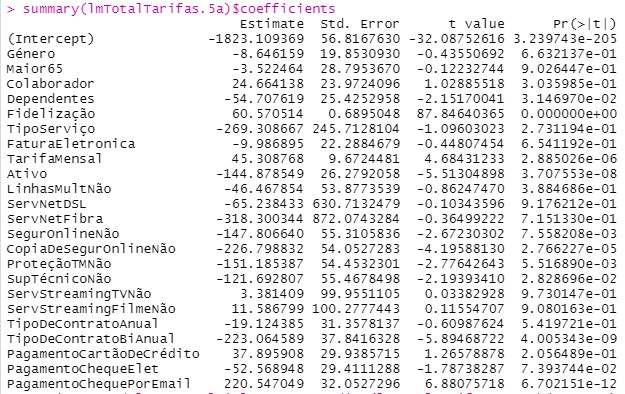
\includegraphics[width=9.5cm]{images/5a_coeficientes.jpg}}
\caption{Resumo de coeficientes do modelo de regressão múltipla.}
\label{5a_coeficientes}
\end{figure}

Na alínea b), utilizamos a função \textbf{rpart} com o método "Anova" para obter a árvore de regressão utilizando o mesmo dataset.

\begin{figure}[htbp]
\centerline{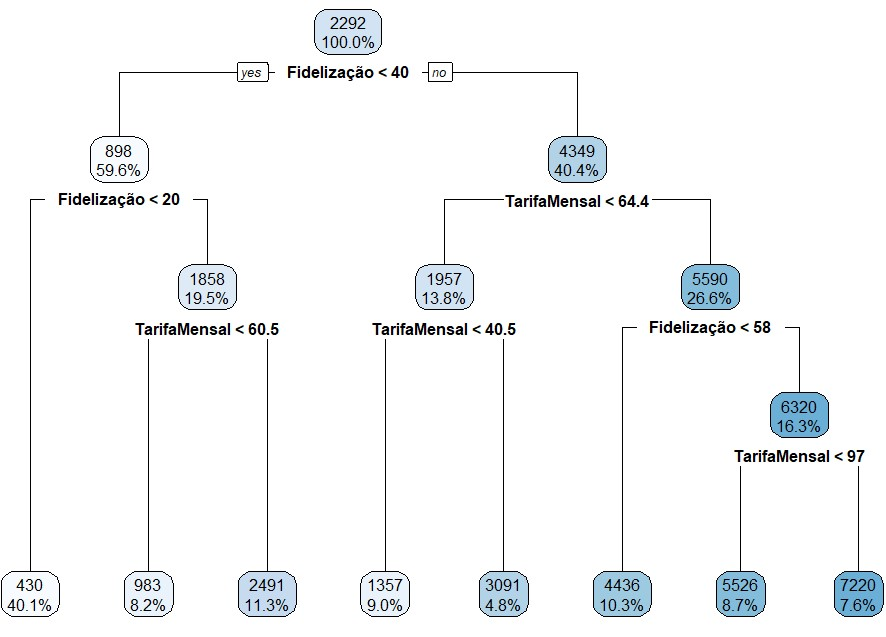
\includegraphics[width=9.5cm]{images/5b_arvore_regressao.jpg}}
\caption{Árvore de regressão.}
\label{5b_arvore_regressao}
\end{figure}

Na alínea c), utilizamos a função \textbf{neuralnet} e o dataset das alíneas anteriores, para gerar uma rede neuronal. Uma vez que pretendemos relacionar um atributo com todos os outros, optamos por colocar o número de nodes igual a 1. Foi testado pela equipa colocar o número de nodes como c(12, 6, 3). Verificou-se que, apesar do valor do mae nao ter diferido muito para apenas 1 nó, o valor do rmse baixou significativamente. Contudo, o grupo optou por utilizar 1 nó. Assim sendo, obtemos a seguinte rede neuronal:

\begin{figure}[htbp]
\centerline{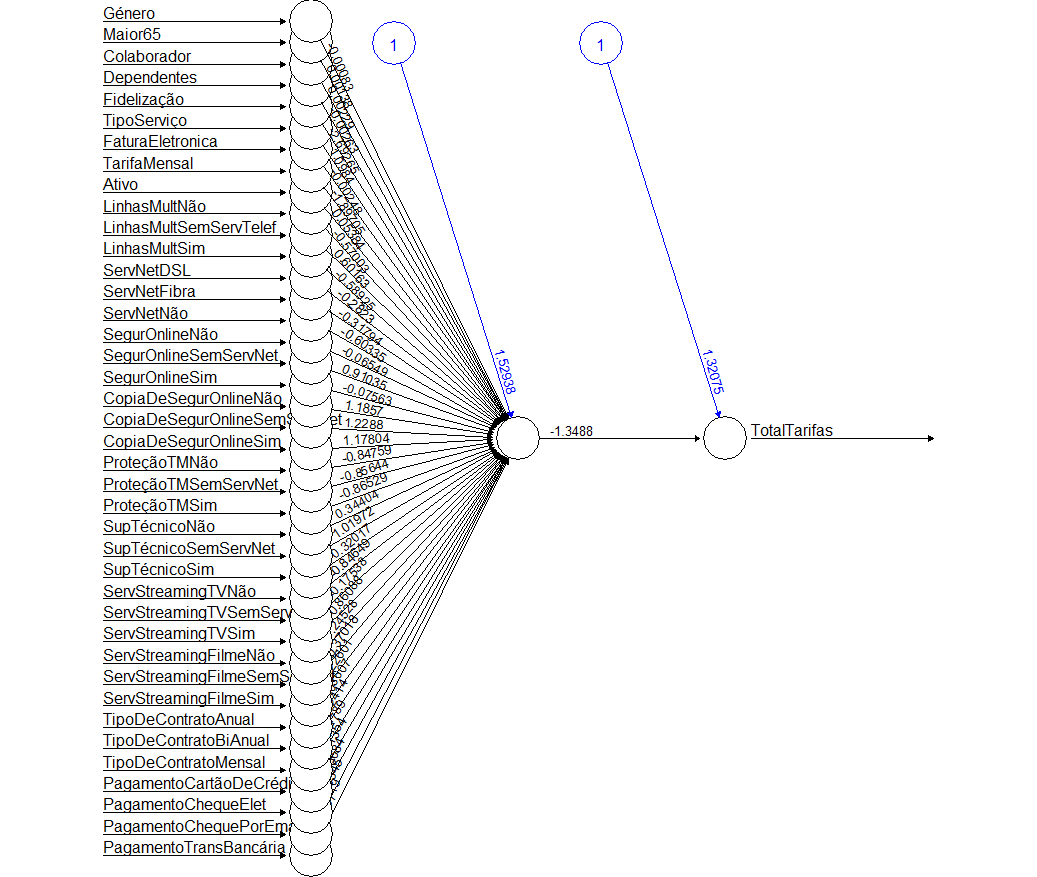
\includegraphics[width=9.5cm]{images/5C_REDE_NEURONAL.JPG}}
\caption{Rede Neuronal}
\label{5C_REDE_NEURONAL}
\end{figure}